%%
%% This is file `sample-sigconf.tex',
%% generated with the docstrip utility.
%%
%% The original source files were:
%%
%% samples.dtx  (with options: `sigconf')
%%
%% IMPORTANT NOTICE:
%%
%% For the copyright see the source file.
%%
%% Any modified versions of this file must be renamed
%% with new filenames distinct from sample-sigconf.tex.
%%
%% For distribution of the original source see the terms
%% for copying and modification in the file samples.dtx.
%%
%% This generated file may be distributed as long as the
%% original source files, as listed above, are part of the
%% same distribution. (The sources need not necessarily be
%% in the same archive or directory.)
%%
%%
%% Commands for TeXCount
%TC:macro \cite [option:text,text]
%TC:macro \citep [option:text,text]
%TC:macro \citet [option:text,text]
%TC:envir table 0 1
%TC:envir table* 0 1
%TC:envir tabular [ignore] word
%TC:envir displaymath 0 word
%TC:envir math 0 word
%TC:envir comment 0 0
%%
%%
%% The first command in your LaTeX source must be the \documentclass
%% command.
%%
%% For submission and review of your manuscript please change the
%% command to \documentclass[manuscript, screen, review]{acmart}.
%%
%% When submitting camera ready or to TAPS, please change the command
%% to \documentclass[sigconf]{acmart} or whichever template is required
%% for your publication.
%%
%%

\documentclass[sigconf]{acmart}

%%
%% \BibTeX command to typeset BibTeX logo in the docs
\AtBeginDocument{%
  \providecommand\BibTeX{{%
    Bib\TeX}}}

%% Rights management information.  This information is sent to you
%% when you complete the rights form.  These commands have SAMPLE
%% values in them; it is your responsibility as an author to replace
%% the commands and values with those provided to you when you
%% complete the rights form.
\setcopyright{acmlicensed}
\copyrightyear{2024}
\acmYear{2024}
\acmDOI{XXXXXXX.XXXXXXX}

%% These commands are for a PROCEEDINGS abstract or paper.
\acmConference[e-Energy '24]{}{June 04--07,
  2024}{Singapore}
%%
%%  Uncomment \acmBooktitle if the title of the proceedings is different
%%  from ``Proceedings of ...''!
%%
%%\acmBooktitle{Woodstock '18: ACM Symposium on Neural Gaze Detection,
%%  June 03--05, 2018, Woodstock, NY}
\acmISBN{978-1-4503-XXXX-X/18/06}


%%
%% Submission ID.
%% Use this when submitting an article to a sponsored event. You'll
%% receive a unique submission ID from the organizers
%% of the event, and this ID should be used as the parameter to this command.
%%\acmSubmissionID{123-A56-BU3}

%%
%% For managing citations, it is recommended to use bibliography
%% files in BibTeX format.
%%
%% You can then either use BibTeX with the ACM-Reference-Format style,
%% or BibLaTeX with the acmnumeric or acmauthoryear sytles, that include
%% support for advanced citation of software artefact from the
%% biblatex-software package, also separately available on CTAN.
%%
%% Look at the sample-*-biblatex.tex files for templates showcasing
%% the biblatex styles.
%%

%%
%% The majority of ACM publications use numbered citations and
%% references.  The command \citestyle{authoryear} switches to the
%% "author year" style.
%%
%% If you are preparing content for an event
%% sponsored by ACM SIGGRAPH, you must use the "author year" style of
%% citations and references.
%% Uncommenting
%% the next command will enable that style.
%%\citestyle{acmauthoryear}

\usepackage{tikz}
\usetikzlibrary{calc,arrows,patterns,intersections}
\usepackage{pgfplots}
\usepackage{bbm}
\usepackage{bm}
\usepackage{adjustbox}

\definecolor{RectangleColor}{RGB}{197,210,180}

%%
%% end of the preamble, start of the body of the document source.
\begin{document}

%%
%% The "title" command has an optional parameter,
%% allowing the author to define a "short title" to be used in page headers.
\title{Energy Intensive Industries Providing Flexibility Services: A Real Case Study of Zinc Galvanizing Process}

%%
%% The "author" command and its associated commands are used to define
%% the authors and their affiliations.
%% Of note is the shared affiliation of the first two authors, and the
%% "authornote" and "authornotemark" commands
%% used to denote shared contribution to the research.

\author{Peter Gade}
\affiliation{%
    \institution{Technical University of Denmark}
    %\institution{IBM Client Innovation Center}
    \city{Kgs. Lyngby}
    \country{Denmark}
}
\email{pega@dtu.dk}

\author{Trygve Skj{\o}tskift}
\affiliation{%
    \institution{IBM Denmark}
    \city{Copenhagen}
    \country{Denmark}
}
\email{Trygve.Skjotskift@ibm.com }

\author{Henrik Bindner}
\affiliation{%
    \institution{Technical University of Denmark}
    \city{Kgs. Lyngby}
    \country{Denmark}
}
\email{hwbi@dtu.dk}

\author{Jalal Kazempour}
\affiliation{%
    \institution{Technical University of Denmark}
    \city{Kgs. Lyngby}
    \country{Denmark}
}
\email{jalal@dtu.dk}

%%
%% By default, the full list of authors will be used in the page
%% headers. Often, this list is too long, and will overlap
%% other information printed in the page headers. This command allows
%% the author to define a more concise list
%% of authors' names for this purpose.
\renewcommand{\shortauthors}{Gade et al.}

%%
%% The abstract is a short summary of the work to be presented in the
%% article.
\begin{abstract}
    Incumbent industrial power consumers can adapt to help balance the power grid. Single-state industry processes are particularly suited for balancing the power grid while earning money and reducing emissions. Using a real-world case study of a zinc galvanizing process, it is shown how modest investments into the power control of the furnace enable flexible provision in two ancillary services, frequency containment reserves (FCR) and manual frequency restoration reserves (mFRR), with a pay-back time potentially within a year. The monetary value of both services is significant with FCR being the preferable service as its impact on the temperature of the zinc is negligible. This paper serves to illustrate how current inflexible demand can become flexible and profitable while aiding the green transition by balancing the power grid.
\end{abstract}

%%
%% The code below is generated by the tool at http://dl.acm.org/ccs.cfm.
%% Please copy and paste the code instead of the example below.
%%
\begin{CCSXML}
    <ccs2012>
    <concept>
    <concept_id>10010583.10010662.10010663.10010666</concept_id>
    <concept_desc>Hardware~Renewable energy</concept_desc>
    <concept_significance>300</concept_significance>
    </concept>
    </ccs2012>
\end{CCSXML}

\ccsdesc[300]{Hardware~Renewable energy}

%%
%% Keywords. The author(s) should pick words that accurately describe
%% the work being presented. Separate the keywords with commas.
\keywords{Demand-side flexibility, thermostatically controlled loads; ancillary services}
%% A "teaser" image appears between the author and affiliation
%% information and the body of the document, and typically spans the
%% page.
% \begin{teaserfigure}
%     \includegraphics[width=\textwidth]{sampleteaser}
%     \caption{Seattle Mariners at Spring Training, 2010.}
%     \Description{Enjoying the baseball game from the third-base
%         seats. Ichiro Suzuki preparing to bat.}
%     \label{fig:teaser}
% \end{teaserfigure}

\received{2 February 2023}
% \received[revised]{12 March 2009}
% \received[accepted]{5 June 2009}

%%
%% This command processes the author and affiliation and title
%% information and builds the first part of the formatted document.
\maketitle

\section{Introduction}

Power prices have increased massively in 2022, and the increasing share of renewable energy stresses the grid to an unprecedented level. In 2022, the Danish transmission operator (TSO), Energinet, spent 2.7 billion on ancillary services, an increase of 1.3 billion from 2021 \cite{energinetOmkostninger}. Energinet expect this cost will only increase further as more renewable, intermittent energy requires more balancing of the power grid.

To facilitate the green transition by using greener technologies to balance the power grid, existing infrastructure can readily be used. In particular, existing power demand can to some degree become flexible, i.e., the power consumption can vary within some thresholds for a certain amount of time as facilitated by an \textit{aggregator}. IBM has created a solution, the Flex Platform, that harness demand-side flexibility to be bid into various ancillary service markets. Power demand in the industrial sector is significant and for simple, single-state industry processes, modest investments can enable them to become flexible.

Single-state processes are characterized by being solely sequential, i.e., the next step occurs after the previous step is done. They are repetitive as well, relatively simple and uncomplicated. Their \textit{state} is often a temperature. They exist everywhere: iron and steel foundries, cooling houses, and a zinc galvanizing operation as shown later (see \cite{paulus2011potential} for an extensive list of energy intensive industry processes). Such processes are prone to become flexible with respect to their power consumption as it requires little to no extra effort or adjustment. Furthermore, it is beneficial and advantageous to harness the flexibility from one big asset as supposed to several hundreds smaller assets.

In the European Union and Denmark, there is an increased focus on $CO_{2}$ \textit{accounting}. Companies, small and large, all need to look thoroughly into their current carbon emissions and especially initiatives that reduce them. Demand-side flexibility is an obvious choice for energy intensive single-state industry processes as it allows them to balance the power grid.\footnote{With the assumption that it would otherwise be provided by fossil fuel power plants.} Other initiatives include energy optimization and energy efficiency, but both have diminishing returns. In Denmark, Energinet has now created a set of rules allowing stochastic demand (or production) to participate with their flexibility \cite{energinet:prequalification}. By allowing for industrial power demand to participate with their flexibility, liquidity in ancillary services increases.

In this work, an industry process is investigated as exemplified by a zinc galvanizing furnace using real data from their process (see Section \ref{sec:zinc_furnace_description} for details). The learnings from this case study readily generalizes to other single-state processes.


\subsection{Research questions}

We investigate how its viable for zinc furnace to adapt for provision of power flexibility through ancillary services such as FCR and mFRR. We do so from a techno-economic perspective while also investigating the temperature impact of delivering flexibility. The research questions addressed are therefore:


\begin{itemize}
    \item Are there incentives for an energy intensive industry process to deliver power flexibility to the grid?
    \item How can it adapt its industry process to provide power flexibility?
    \item Are ancillary services such as FCR and mFRR suited for such a process?
    \item What is the monetary impact of temperature thresholds?
\end{itemize}

The first question is answered by qualitatively assessing the overall case study, combining carbon emission and monetary incentives. The second question is answered by thoroughly investigating the operational baseline power consumption profile of the zinc furnace, and giving recommendations on the \textit{investments} needed to cater for power flexibility provision. The third question looks at the two revenue streams for the zinc furnace's flexibility potential: FCR with a small but fast energy delivery and mFRR with a large but slow energy delivery. The fourth question is answered by conducting a sensitivity analysis on allowed temperature deviation of the zinc together with a qualitative comparison of FCR and mFRR.


\subsection{Investments should facilitate power flexibility}

New investments into equipment and improvements in the industry process can be tailored to facilitate power flexibility. For example, instead of relying on mechanical relay switches for power lines, frequency transformers or thyristors can be used instead for a modest marginal extra cost. The pay-back time for such an investment should ideally be within a few years, and other benefits could potentially be exploited as well, e.g., better feed forward planning.

% Early indications for the owner of the zinc furnace indicate a one-time cost of 0.5 mio. DKK into equipment that allows for granular power control to the furnace.

\subsection{Value streams from power flexibility: FCR and mFRR}

Power consumption can potentially be flexible if the underlying operation has a  degree of freedom. For example, power consumption to heat up zinc can be controlled as long as the temperature of the zinc is within some pre-specified thresholds. These determine the degrees of freedom in the operation. For the zinc furnace, the lower temperature threshold specify solidification of molten zinc which can have a detrimental impact as it can crack the furnace wall.

The ability to deviate from the operational baseline power consumption can be monetized by participating in ancillary services such as FCR and mFRR. Furthermore, if these services are normally delivered by fossil fuel power plants, these are partly displaced and a CO$_{2}$ emission reduction is realized.

The demand for FCR and mFRR is expected to increase significantly in Denmark due to massive penetration of intermittent solar and wind energy in the power grid \cite{energinet:scenario_report_2022}. Hence, both markets provide medium to long-term opportunities for monetizing power flexibility.

% In our work, we look only at monetary value and feasibility from FCR and mFRR as it is not yet clear how the CO$_{2}$ emissions impact can be quantified.

\subsection{Literature review}

Many studies have investigated demand-side flexibility. While most have focused on flexibility from residential households in an aggregated portfolio, some have also looked at industry processes with a significant electric energy consumption. For example, \cite{paulus2011potential} show the huge potential for energy intensive industry processes to provide balancing reserves. According to the authors knowledge, none specifically look at single-state industrial processes in a real-life setting while addressing their incentives to deliver power flexibility.

Of these, freezers have been investigated thoroughly both with respect to mathematical representation \cite{pedersen2016improving}  and as a source of flexibility \cite{sossan2016grey}, \cite{o2013modelling}, \cite{de2019leveraging}, \cite{misaghian2022fast}, \cite{vrettos2016fast}. Freezers are potentially a great source of flexibility because of the thermal inertia in the frozen food. However, supermarket freezers are complicated systems in which individual freezer displays are dependent of each other as they are fed cold air from the same compressor rack. Furthermore, there are many food regulations that complicate control of freezers with respect to allowed temperature deviations.

Much work has also gone into understanding heat dynamics of medium-large buildings \cite{thilker2021non} in order to operate them intelligently with respect to electricity prices and the grid \cite{contreras2018tractable}, \cite{finck2018quantifying}. However, this operation also comes with complexity in terms of control with potentially many different (dependent) heterogeneous assets such as ventilation units, heat pumps, water tanks, and heating units. Many single-state industrial processes are likely better suited for flexibility provision as they are more simple and easily modifiable.

In \cite{mallapragada2023decarbonization}, it is argued that energy intensive chemical processes can benefit from investments into electrification. The payback time of the investments can be reduced significantly by exploiting the capabilities of power electronics to deliver balancing services to the grid. Likewise, it is shown in \cite{samani2022flexible} how a chemical process can deliver FCR to the grid while still maintaining the same operational quality.

In \cite{junker2020stochastic}, a water tower is characterized using stochastic differential equations for best planning how water should be pumped in relation to spot prices. Although not specifically for ancillary services, this serves as an illustrative example how operational control can benefit from knowledge of electricity prices in a fairly simple industry process.

The most simple mathematical model of a thermostatically controlled load (TCL), was presented in Hao et. al. \cite{hao2014aggregate}. Here, a first-order model with two terms fully characterized the TCL: a term that explains temperature losses due to temperature differences and a term that explains temperature gains due to a power source. We expand upon this model in this paper, using instead a 4$^{\text{th}}$ order model to characterize a zinc furnace.

While a simple, linear model is used for modelling FCR provision in this paper, the model introduced in \cite{gade2023load} is used to model mFRR provision.



\subsection{Our contribution}

For a real-life energy intensive industry process using real data, we investigate if there is any incentive to provide power flexibility or to invest in equipment for the enablement of flexibility provision.

Specifically, we investigate such a case using actual (anonymized) data collected from 2022 and price- and frequency data for 2021-2023. We describe the process in detail and show how it can be adapted to cater for power flexibility by switching from ON/OFF power control to continuous power control.

The monetary value from power flexibility is shown for FCR and mFRR provision in DK1\footnote{DK1 is the western part of Denmark and shares the same frequency as continental Europe.} in Denmark. We provide an upper bound of flexibility earnings using a full hindsight optimization of each service and its impact on the temperature, i.e., the state of the industry process, is analyzed. We discuss and show how the allowed degrees of freedom in the temperature deviation impact the monetary value of flexibility provision.

Our case study naturally generalizes to many similar single-state industry processes seen in, e.g., foundries where the state in question is temperature related.

% {\color{red}Should we instead provide paper structure here??}

The rest of the paper is organized as follows. First, we describe the process in detail and show how the thermal characteristics of the zinc furnace can be formulated. Second, we show how investments into a more granular, continuous control of the power supply to the furnace enables it to deliver power flexibility. Two quite different ancillary services are targeted: FCR and mFRR. For both, full-hindsight optimizations are provided to compute upper-bound potentials. Lastly, an analysis of the zinc temperature's impact on the flexibility potential is carried out.


\section{Adapting a single-state industry process to provide flexibility}\label{sec:zinc_furnace_description}

In this section, the zinc galvanizing process is described in detail along with its ability to provide power flexibility by converting to a continuous control mechanism.

We first describe how the temperature of the molten zinc can be characterized using state-space models. Then it is shown how this model can be used for subsequent simulation of continuous control. Afterwards, it it shown how power flexibility can be monetized in FCR and mFRR.

\subsection{Characterizing a zinc furnace as a TCL}



\subsubsection{Description of zinc furnace in a galvanizing process}

The industry process exemplified in this paper is a galvanization process, in which the authors have kindly been allowed to see and learn about by the owner, DOT Nordic. Steel elements are galvanized by lowering them into a molten zinc furnace at a high temperature setpoint. As seen in Figure \ref{fig:furnace_schematic_tikz}, the furnace is heated up by resistive elements placed on the sides of the furnace (in an inner cavity). The upper and lower zones of the furnace are controlled separately with $P^{\text{u}}$ and $P^{\text{l}}$ representing the power supplied to the upper and lower zone, respectively. Temperature sensors are placed in each zone at the end of the furnace on the wall as denoted by $T^{\text{wu}}$ and $T^{\text{wl}}$, hence the actual zinc temperatures, $(T^{\text{zu}})$ and $(T^{\text{zl}})$, are latent, unobserved states. The lid of the furnace is removed when lowering steel into the furnace.

\begin{figure}[t]
    \centering
    \documentclass[crop,tikz]{standalone}
\usepackage[usenames]{color} %used for font color
\usepackage{amssymb} %maths
\usepackage{amsmath} %maths
\usepackage[utf8]{inputenc} %useful to type directly diacritic characters
\usepackage{tikz}
\usetikzlibrary{calc,arrows,patterns,intersections}
\usetikzlibrary{shapes.multipart}
\usepackage{pgfplots}
\usepgfplotslibrary{fillbetween}
\pgfmathdeclarefunction{gauss}{2}{%
  \pgfmathparse{1/(#2*sqrt(2*pi))*exp(-((x-#1)^2)/(2*#2^2))}%
}
\begin{document}

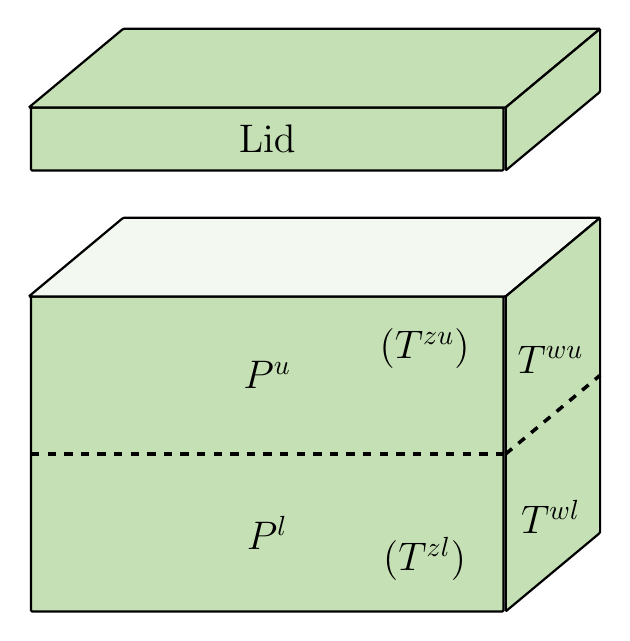
\begin{tikzpicture}
  \definecolor{CUBE}{RGB}{197,224,180};
  % Settings
  \coordinate (CenterPoint) at (0,0);
  \def\width{6.0cm};
  \def\height{4.0cm};
  \def\textborder{1.0cm};
  \def\xslant{1.2cm};
  \def\yslant{1.0cm};
  \def\rounding{0.4pt};
  % Drawing
  \node[thick, draw,
    minimum height  = \height,
    minimum width   = \width,
    text width      = {\width-1*\textborder},
    align           = center,
    fill            = CUBE,
    rounded corners = \rounding]
  at (CenterPoint) {}; % TEXT HERE?

  \draw[name path=HorizontalDashedLine, dashed, line width=0.45mm, black]%
  ($(CenterPoint) + (-\width/2., 0)$) -- ($(CenterPoint) + (\width/2., 0)$);

  % "3D" top
  \draw [rounded corners = \rounding, thick, fill=CUBE!20] %
  ($(CenterPoint) + (-\width/2. - 2*\rounding, \height/2.)$) -- %
  ($(CenterPoint) + (-\width/2. + \xslant - 2*\rounding, \height/2. + \yslant)$) -- %
  ($(CenterPoint) + (\width/2. + \xslant + 2*\rounding, \height/2. + \yslant)$) -- %
  ($(CenterPoint) + (\width/2. + 2*\rounding, \height/2.)$) -- %
  cycle;
  % "3D" side
  \draw [rounded corners = \rounding, thick, fill=CUBE] %
  ($(CenterPoint) + (\width/2. + \xslant + 2*\rounding, \height/2. + \yslant)$) -- %
  ($(CenterPoint) + (\width/2. + 2*\rounding, \height/2.)$) -- %
  ($(CenterPoint) + (\width/2. + 2*\rounding, -\height/2.)$) -- %
  ($(CenterPoint) + (\width/2. + \xslant + 2*\rounding, -\height/2. + \yslant)$) -- %
  cycle;

  \coordinate (CenterPointLid) at (0,4);
  \node[thick, draw,
    minimum height  = \height*0.2,
    minimum width   = \width,
    text width      = {\width-1*\textborder},
    align           = center,
    fill            = CUBE,
    rounded corners = \rounding]
  at (CenterPointLid){\Large Lid};

  \draw [rounded corners = \rounding, thick, fill=CUBE] %
  ($(CenterPointLid) + (-\width/2. - 2*\rounding, 0.2*\height/2.)$) -- %
  ($(CenterPointLid) + (-\width/2. + \xslant - 2*\rounding, 0.2*\height/2. + \yslant)$) -- %
  ($(CenterPointLid) + (\width/2. + \xslant + 2*\rounding, 0.2*\height/2. + \yslant)$) -- %
  ($(CenterPointLid) + (\width/2. + 2*\rounding, 0.2*\height/2.)$) -- %
  cycle;

  \draw [rounded corners = \rounding, thick, fill=CUBE] %
  ($(CenterPointLid) + (\width/2. + \xslant + 2*\rounding, 0.2*\height/2. + \yslant)$) -- %
  ($(CenterPointLid) + (\width/2. + 2*\rounding, 0.2*\height/2.)$) -- %
  ($(CenterPointLid) + (\width/2. + 2*\rounding, -0.2*\height/2.)$) -- %
  ($(CenterPointLid) + (\width/2. + \xslant + 2*\rounding, -0.2*\height/2. + \yslant)$) -- %
  cycle;

  \draw[name path=HorizontalDashedLineSide, dashed, line width=0.45mm, black]%
  ($(CenterPoint) + (\width/2. + 2*\rounding, 0)$) -- ($(CenterPoint) + (\width/2. + \xslant + 2*\rounding, + \yslant)$);

  % wall annotations
  \node at ($(CenterPoint) + (\width/2. + \xslant/2., \yslant*1.2)$) % 
  {\Large $T^{\text{wu}}$};
  \node at ($(CenterPoint) + (\width/2. + \xslant/2., -\yslant*0.8)$) % 
  {\Large $T^{\text{wl}}$};

  % zinc annotations
  \node at ($(CenterPoint) + (\width/3., \height/3)$) % 
  {\Large $(T^{\text{zu}})$};
  \node at ($(CenterPoint) + (\width/3., -\height/3)$) % 
  {\Large $(T^{\text{zl}})$};

  % power annotations
  \node at ($(CenterPoint) + (0, \height/4)$) % 
  {\Large $P^{\text{u}}$};
  \node at ($(CenterPoint) + (0, -\height/4)$) % 
  {\Large $P^{\text{l}}$};


\end{tikzpicture}

\end{document}
    \caption{Schematic of the zinc furnace. Resistive elements are places on both sides of the furnace in inner cavities for both zones. The power consumptions of the resistive elements are denoted $P^{\text{u}}$ and $P^{\text{l}}$. At the end of the furnace, two temperature sensors are located, measuring the wall temperatures, $T^{\text{wu}}$ and $T^{\text{wl}}$. Hence, the actual zinc temperatures are unobserved. The lid is off during the galvanizing process. QU1 and QU2 are the contactors for the upper zone, and QL3 and QL4 are the contactors for the lower zone.}
    \Description{Schematic of zinc furnace.}
    \label{fig:furnace_schematic_tikz}
\end{figure}

Figure \ref{fig:data_visualization} shows the anonymized\footnote{The scale of the temperature has been anonymized.} one-minute resolution data provided. The upper panel shows the power consumption of the lower and upper zones, respectively, and the total consumption as well. It is clearly seen how two regimes are immediately identified: One where the lid is on the furnace and the power consumption is quite low, and one where the lid is off corresponding to a high power consumption due to direct temperature losses to the ambient. In both the middle and bottom panel of Figure \ref{fig:data_visualization}, the temperature dynamics behave differently in either regime: When the lid is on, the temperature varies slowly while it varies rapidly when the lid is off. Furthermore, the temperature dynamics are generally slower in the lower zone of the furnace (bottom panel), and its temperature setpoint is also a bit lower. The ON/OFF control of the power consumption to the two zones are visualized by the state of four contactors - two for each zone - as seen in the middle and bottom panel. The control logic is simple for a given zone: one contactor is switched ON (QU1 $=1$ or QL3 $=1$) when the temperature goes belows a pre-specified threshold, and the other one is turned ON (QU2 $=1$ or QL4 $=1$) as well if the temperature declines further below another pre-specified threshold. Exactly the same logic applies when the temperature rises above two pre-specified upper thresholds. This logic is statically programmed for both zones independently.

\begin{figure}[t]
    \centering
    \includegraphics[width=\columnwidth]{figures/data_visualization.png}
    \caption{\textbf{Top}: Power consumption for lower and upper zone as well as total consumption. \textbf{Middle}: Temperature and contactor switches in upper zone. \textbf{Bottom}: Temperature and contactor switches in lower zone.}
    \Description{Plot of raw zinc furnace power and temperatuer data.}
    \label{fig:data_visualization}
\end{figure}

\subsubsection{Thermal modelling of zinc furnace}

To model the temperature dynamics in both zones, a fourth-order state-space model is used (\ref{eq:StateSpaceModel}):

\begin{subequations}\label{eq:StateSpaceModel}
    \begin{align}
        T^{\text{zu}}_{t+1} & = T^{\text{zu}}_{t} + dt \cdot \frac{1}{C^{\text{zu}}}\Bigl( \frac{1}{R^{\text{zuzl}}} (T^{\text{zl}}_{t} - T^{\text{zu}}_{t}) \notag                                     \\ & \mspace{5mu} + \frac{1}{R^{\text{wz}}} (T^{\text{wu}}_{t} - T^{\text{zu}}_{t}) \Bigr) \label{eq1:StateSpaceModel} \\
        T^{\text{zl}}_{t+1} & = T^{\text{zl}}_{t} + dt \cdot \frac{1}{C^{\text{zl}}}\Bigl( \frac{1}{R^{\text{zuzl}}} (T^{\text{zu}}_{t} - T^{\text{zl}}_{t}) \notag                                     \\ & \mspace{5mu} + \frac{1}{R^{\text{wz}}} (T^{\text{wl}}_{t} - T^{\text{zl}}_{t}) \Bigr) \label{eq2:StateSpaceModel} \\
        T^{\text{wu}}_{t+1} & = T^{\text{wu}}_{t} + dt \cdot \frac{1}{C^{\text{wu}}}\Bigl( (1-\mathbbm{1}^{\text{lid}}) \frac{1}{R^{\text{wua},\text{off}}} (T^{\text{a}} - T^{\text{wu}}_{t}) \notag + \\ & \mspace{5mu} \mathbbm{1}^{\text{lid}} \frac{1}{R^{\text{wua},\text{on}}} (T^{\text{a}} - T^{\text{wu}}_{t}) + \frac{1}{R^{\text{ww}}} (T^{\text{wl}}_{t} - T^{\text{wu}}_{t}) \notag \\ & \mspace{5mu} + \frac{1}{R^{\text{wz}}} (T^{\text{zu}}_{t} - T^{\text{wu}}_{t}) + p^{\text{u}}_{t} \Bigr) \label{eq3:StateSpaceModel} \\
        T^{\text{wl}}_{t+1} & = T^{\text{wl}}_{t} + dt \cdot \frac{1}{C^{\text{wl}}}\Bigl( \frac{1}{R^{\text{wla}}} (T^{\text{a}} - T^{\text{wl}}_{t}) \notag                                           \\ & \mspace{5mu} + \frac{1}{R^{\text{ww}}} (T^{\text{wu}}_{t} - T^{\text{wl}}_{t}) + \frac{1}{R^{\text{wz}}} (T^{\text{zl}}_{t} - T^{\text{wl}}_{t}) + p^{\text{l}}_{t} \Bigr) \label{eq4:StateSpaceModel}
    \end{align}
\end{subequations}

Here, (\ref{eq1:StateSpaceModel}) and (\ref{eq3:StateSpaceModel}) represent the (latent) temperature of the zinc in the upper and lower zone, respectively. For both, there is a heat exchange between the furnace walls and the other zinc zone. In (\ref{eq3:StateSpaceModel}), the temperature dynamics of the upper part of the wall of the zinc furnace is shown. It depends on the heat loss to the ambient temperature, $T^{\text{a}}$, heat exchange with the lower wall, $T^{\text{wl}}$, with the zinc in the upper zone, $T^{\text{zu}}$, and the heat added from the resistive elements in the upper zone, $p^{\text{u}}$. Furthermore, there are two different resistance coefficients, $R^{\text{wua},\text{off}}$ and $R^{\text{wua},\text{on}}$, depending on whether the lid is on ($ \mathbbm{1}^{\text{lid}} = 1$) or off ($ \mathbbm{1}^{\text{lid}} = 0$). The index $t$ represents a minute and $dt = \frac{1}{60}$ is the timestep.

The procedure of parameter estimation in (\ref{eq:StateSpaceModel}) is shown in Appendix \ref{app:parameter-estimation}


\subsubsection{Going from ON/OFF control to steady-state control}

As seen in Figure \ref{fig:data_visualization}, the power consumption is rather unpredictable and varying with the ON/OFF control mechanism. Hence, it is difficult to predict the operational baseline power consumption of the zinc furnace. Therefore, if the furnace should benefit from providing flexibility to the power grid through ancillary services, it is necessary to change the control structure to a more granular one.\footnote{In theory, the furnace can still participate in the current market structure of mFRR with 1-hour blocks if it is part of a bigger portfolio that can compensate for its ON/OFF behavior.}

Using the model in (\ref{eq:StateSpaceModel}), we can estimate the steady-state power consumption for both regimes, i.e., when the lid is on and off:

% p_{u}^{\text{Base}} & = \frac{T^{\text{u},\text{sp}} - T^{\text{a}}}{R^{\text{wua},1}}  + \frac{T^{\text{u},\text{sp}}-T^{\text{l},\text{sp}}}{R^{\text{ww}}} \label{eq1:steady-state-power} \\
% p^{\text{u},\text{SS},2} & = \frac{T^{\text{u},\text{sp}} - T^{\text{a}}}{R^{\text{wua},2}} + \frac{T^{\text{u},\text{sp}}-T^{\text{l},\text{sp}}}{R^{\text{ww}}} \label{eq2:steady-state-power}  \\
% p^{\text{l},\text{SS}}   & = \frac{T^{\text{l},\text{sp}} - T^{\text{a}}}{R^{\text{wla}}} - \frac{T^{\text{u},\text{sp}}-T^{\text{l},\text{sp}}}{R^{\text{ww}}} \label{eq3:steady-state-power}

\begin{equation}\label{eq1:steady-state-power}
    p^{\text{l},\text{Base}} = \frac{T^{\text{l},\text{sp}} - T^{\text{a}}}{R^{\text{wla}}} - \frac{T^{\text{u},\text{sp}}-T^{\text{l},\text{sp}}}{R^{\text{ww}}}
\end{equation}

\begin{equation}\label{eq2:steady-state-power}
    p^{\text{u},\text{Base}}   =
    \begin{cases}
        \frac{T^{\text{u},\text{sp}} - T^{\text{a}}}{R^{\text{wua},\text{off}}}  + \frac{T^{\text{u},\text{sp}}-T^{\text{l},\text{sp}}}{R^{\text{ww}}}, & \text{if} \ \text{Lid is on}  \\
        \frac{T^{\text{u},\text{sp}} - T^{\text{a}}}{R^{\text{wua},\text{on}}} + \frac{T^{\text{u},\text{sp}}-T^{\text{l},\text{sp}}}{R^{\text{ww}}},   & \text{if} \ \text{Lid is off} \\
    \end{cases}
\end{equation}

Here, $T^{\text{l},\text{sp}}$ and $T^{\text{u},\text{sp}}$ are the pre-specified setpoints in the lower and upper zone, respectively. $p^{\text{l},\text{Base}}$ is the steady-state power consumption for the lower zone, and $p^{\text{u},\text{Base}}$ is the steady-state power consumption for the upper zone which takes two values depending of whether the lid is on or off.

Appendix \ref{app:steady-state-simulation} shows a simulation of (\ref{eq:StateSpaceModel}) using (\ref{eq1:steady-state-power}) and (\ref{eq2:steady-state-power}). The purpose of the steady-state operation is to highlight the benefit of flexibility provision from a more predictable, operational baseline consumption while the intricacies of the control logic is not investigated further here.

Furthermore, other benefits of using a more continuous power control include more optimal use of the heat in the furnace by being able to integrate the dipping schedule to the power consumption. Hence, smarter feed forward planning of the lid can be achieved and made possible by utilizing continuous power control.

Early indications from the owner of the zinc furnace show a one-time cost of 0.5 mil. DKK into equipment and power electronics that allows for granular power control.

\subsection{FCR}

FCR is the fastest responding ancillary service in DK1 in Denmark. Power must be adjusted according to frequency deviations around $\pm 200$ mHz from 50 Hz \cite{energinet:prequalification}. The service is delivered primarily by thermal power plants and batteries, but flexible demand can potentially also deliver FCR; either by control of individual assets or from an aggregation of multiple assets that can be turned ON/OFF in a manner that adheres to the frequency response requirements.

The service is bought by the Danish TSO in 4-hour blocks in one auction for the upcoming day. The auction starts at 8:00 AM the day before delivery. Flexibility providers receive the marginal price of the auction as payment for providing capacity.

\begin{figure}\label{fig:timeline}
    \begin{adjustbox}{width=\columnwidth}
        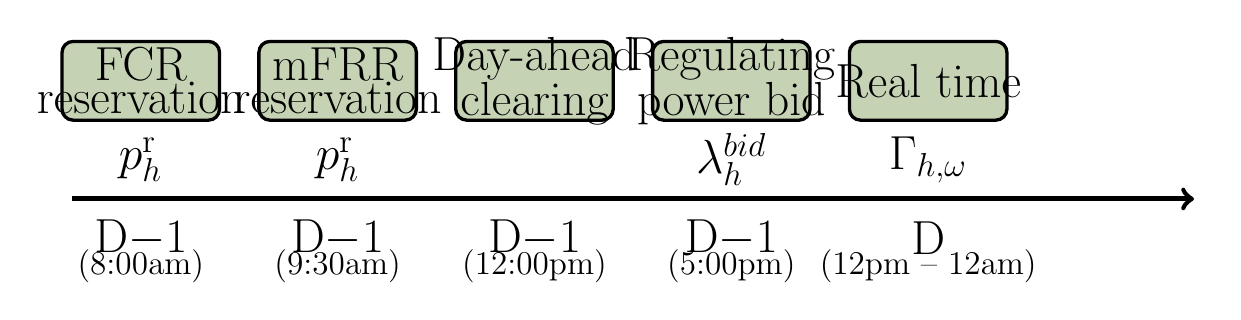
\begin{tikzpicture}[scale=0.50,every text node part/.style={align=center}]

  \draw[rounded corners, fill=RectangleColor, very thick] (-5, 1) rectangle (-1, 3) node[midway]{\LARGE FCR \\ \LARGE reservation};
  \node at (-3,0) {\LARGE  $p_{h}^{\rm{r}}$};
  \node at (-3,-2) {\LARGE D$-$1};
  \node at (-3,-2.7) {\large (8:00am)};
  
  \draw[rounded corners, fill=RectangleColor, very thick] (0, 1) rectangle (4, 3) node[midway]{\LARGE mFRR \\ \LARGE reservation};
  \node at (2,0) {\LARGE  $p_{h}^{\rm{r}}$};
  \node at (2,-2) {\LARGE D$-$1};
  \node at (2,-2.7) {\large (9:30am)};


  \draw[rounded corners, fill=RectangleColor, very thick] (5, 1) rectangle (9, 3) node[midway]{\LARGE Day-ahead \\ \LARGE clearing};
  \node at (7,-2) {\LARGE D$-$1};
  \node at (7,-2.7) {\large (12:00pm)};

  \draw[rounded corners, fill=RectangleColor, very thick] (10, 1) rectangle (14, 3) node[midway]{\LARGE Regulating  \\ \LARGE power bid};
  \node at (12,0) { \LARGE $\lambda_{h}^{\text{bid}}$};
  \node at (12,-2) {\LARGE D$-$1};
  \node at (12,-2.7) {\large (5:00pm)};

  \draw[rounded corners, fill=RectangleColor, very thick] (15, 1) rectangle (19, 3) node[midway]{\LARGE Real time};
  \node at (17,0) {\LARGE $\Gamma_{h,\omega}$};
  % {\LARGE $\Bigl( \bm{p}^{\rm{r},\uparrow}, \bm{\lambda}_{\omega}^{\text{bid}}, \bm{p}_{\omega}^{b,\uparrow}, \bm{p}_{\omega}^{b,\downarrow}, \bm{s}_{\omega}, \bm{T}_{\omega}^{c}, \bm{T}_{\omega}^{f}, \notag \\ \quad & \quad \bm{T}_{\omega}^{c, B}, \bm{T}_{\omega}^{f,B}, \bm{\phi}_{\omega}, \bm{g}_{\omega} \Bigr)$};
  \node at (17,-2) {\LARGE D};
  \node at (17,-2.7) {\large (12pm -- 12am)};


  % Right arrow
  \node (source) at (0-5, -1) {};
  \node (destination) at (24,-1){};
  \draw[->, line width=0.65mm, black](source)--(destination);


\end{tikzpicture}
    \end{adjustbox}
    \caption{Timeline of variables for bidding into FCR and mFRR. For FCR, the reservation bid for day $D$ is made the before at 8:00am, and the real-time power $\bm{p}^{q}$ is determined from the bids. For mFRR, reservation bids are made at 9:30am in $D-1$ while regulating power bids are submitted at 5:00pm. Real-time variables for mFRR are denoted by $\Gamma_{h}$.}
    \Description{Timeline of variables related to bidding into FCR and mFRR}
\end{figure}


\subsection{mFRR}

mFRR is an ancillary service operated by the TSO. It is the last service deployed after a frequency drop, and the energy content delivered to the grid can be several MW. In DK1 in Denmark, the TSO procures around 600 MW of mFRR \cite{energinet:scenario_report_2022}.

As described in \cite{gade2023load}, procurement of mFRR reserves happens before the day-ahead market clearing, and the subsequent balancing bid happens after the day-ahead market clearing. mFRR providers are paid at the marginal price according to the capacity they offer. In real-time, activation of reserves happens when the TSO demands it which leads to a balancing price higher than the spot price. mFRR providers are paid according to the amount they activate and penalized if they do not deliver their promised capacity. For TCLs, such as a zinc furnace, there will be an inevitable rebound which requires additional energy.

Appendix \ref{app:market-prices} shows historical prices for 2021-2023 for FCR and mFRR as well as spot prices.


\section{Optimization models}

The optimization models for FCR and mFRR are presented in this section. First, the FCR model is presented. Second, the mFRR model is presented in compact form. Both models are deterministic with full hindsight on prices. We thus provide an upper bound in the flexibility potential which is useful to know when deciding to make investments that enables power flexibility provision. Hence, if the upper bound potential is not attractive, then investments should not be made.

\subsection{FCR}

The linear optimization model for FCR reserve bidding and activation is shown in compact form in (\ref{P1:compact_model_fcr}) with bold indicating time vectors. The objective in (\ref{P1:eq1}) maximizes revenue from capacity payments and minimizes penalties. The aggregator incurs a penalty cost of at $\lambda^{\text{Pen}}$ DKK/kWh whenever the reserve, $\bm{p}^{r}$, cannot be met.

Variables related to bidding capacity and penalty are indexed by hours, $\bm{\Gamma}_{h}$, and variables related to real-time control are indexed by minute, $\bm{\Gamma}_{t}$.

% # TODO: be aware of different time scale: minute vs hourly!!
\begin{subequations}\label{P1:compact_model_fcr}
    \begin{align}
        \underset{\bm{\Gamma}_{h},\bm{\Gamma}_{t}}{\textrm{max}} \quad & \bm{p}^{r} \bm{\lambda}^{\text{FCR}} - \bm{s}\lambda^{\text{Pen}} \label{P1:eq1}
        \\
        s.t \quad                                                      & q(\bm{\Gamma}_{h}, ) \leq 0 \label{P1:eq2}                                                                                                                    \\
        \quad                                                          & \text{State-space model in } (\ref{eq:StateSpaceModel}), \label{P1:eq8}                                                                                       \\
        \quad
                                                                       & \bm{\Gamma}_{h} = \Bigl( \bm{p}^{r}, \bm{s} \Bigr) \in \mathbb{R}  \label{P1:eq9}                                                                             \\
        \quad
                                                                       & \bm{\Gamma}_{t} = \Bigl( \bm{p}, \bm{p}^{q}, \bm{s}^{q, \prime}, \bm{T}^{\text{z},q}, \bm{T}^{\text{w},q} \Bigr) \in \mathbb{R}, \ \forall{q} \label{P1:eq10}
    \end{align}
\end{subequations}

The inequality constraints in (\ref{P1:eq2}) are shown in (\ref{P1:constraints}) below. Since FCR is a symmetric service, auxiliary variables $\bm{s}^{\prime}$ are introduced to account for the power not delivered as shown in (\ref{P1:co3})-(\ref{P1:co4}). The superscript $q$ denotes the two zones $\{l, u\}$ in the zinc furnace, and the total reserve from the zinc furnace is simply the sum of these as seen in (\ref{P1:co6})-(\ref{P1:co7}).

\begin{subequations} \label{P1:constraints}
    \begin{align}
              & \bm{p}^{q} = \bm{F} \bm{p}^{q,r} + \bm{s}^{q, \prime} + \bm{P}^{q, \text{Base}}, \quad \forall{q}  \label{P1:co2} \\
        \quad & \bm{s}^{q} \geq \bm{s}^{q, \prime}, \quad \forall{q}  \label{P1:co3}
        \\
        \quad & \bm{s}^{q} \geq -\bm{s}^{q,\prime}, \quad \forall{q}  \label{P1:co4}
        \\
        \quad & \bm{p}^{q,r} \leq \bm{P}^{q,\text{Base}} , \quad \forall{q} \label{P1:co8}
        \\
        \quad & \bm{p} = \sum_{q} \bm{p}^{q}   \label{P1:co5}                                                                     \\
        \quad & \bm{p}^{r} = \sum_{q} \bm{p}^{q,r}   \label{P1:co6}                                                               \\
        \quad & \bm{s} = dt \sum_{q} \bm{s}^{q}   \label{P1:co7}
    \end{align}
\end{subequations}

The parameter $\bm{F}$ is normalized between -1 and 1 depending on the frequency such that it represents the normalized response required \cite{energinet:prequalification}:

\begin{equation}
    F_{t} =
    \begin{cases}
        -1,                             & \text{if}\ F_{t} \leq 49.8\ \text{Hz}                                          \\
        \frac{F_{t}-50+0.02}{0.2-0.02}, & \text{if}\ F_{t} \leq 49.98\ \text{Hz}\ \text{and}\ F_{t} \geq 49.8\ \text{Hz} \\
        \frac{F_{t}-50-0.02}{0.2-0.02}, & \text{if}\ F_{t} \leq 50.2\ \text{Hz}\ \text{and}\ F_{t} \geq 50.02\ \text{Hz} \\
        1,                              & \text{if}\ F_{t} \geq 50.2 \text{Hz}                                           \\
    \end{cases}
\end{equation}

\subsection{mFRR}

The optimization model for mFRR is identical to \cite{gade2023load} with no scenarios and a different state-space model (\ref{eq:StateSpaceModel}) as shown in (\ref{P1:compact_model_mfrr}).

\begin{subequations}\label{P1:compact_model_mfrr}
    \begin{align}
        \underset{\bm{p}^{\rm{r}}, \bm{p}^{q,\rm{r}}, \bm{\lambda}^{\rm{bid}}, \bm{\Gamma}}{\text{Maximize}} \  & f(\bm{p}^{\rm{r}}, \bm{p}^{q,\rm{r}}) + g(\bm{\Gamma}) \label{P1:eq1_mfrr}
        \\
        \text{s.t.} \                                                                                           & h(\bm{p}^{\rm{r}}, \bm{p}^{q,\rm{r}}, \bm{\lambda}^{\rm{bid}}, \bm{\Gamma}) \leq 0, \label{P1:eq2_mfrr}                                              \\
        \                                                                                                       & \text{State-space model } (\ref{eq:StateSpaceModel}),  \label{P1:eq3_mfrr}
        \\
        \                                                                                                       & \bm{T}^{\text{z},q}, \bm{T}^{\text{w},q} \in \mathbb{R}, \forall{q} \label{P1:eq4_mfrr}
        \\
        \                                                                                                       & \bm{T}^{\text{z},q,\text{Base}}, \bm{T}^{\text{w},q,\text{Base}}, \in \mathbb{R}, \ \forall{q} \label{P1:eq5_mfrr}
        \\
        \                                                                                                       & \Bigl( \bm{p}, \bm{p}^{q}, \bm{p}^{\rm{r}}, \bm{p}^{q,\rm{r}}, \bm{\lambda}^{\rm{bid}}, \bm{p}^{\rm{b},\uparrow}, \bm{p}^{\rm{b},\downarrow}, \notag \\ & \bm{p}^{q,\rm{b},\uparrow}, \bm{p}^{q,\rm{b},\downarrow}, \bm{s}, \bm{s}^{q}, \bm{\phi} \Bigr) \in \mathbb{R}^{+}, \ \forall{q}  \label{P1:eq6_mfrr}
        \\
        \                                                                                                       & \Bigl( \bm{g}, \bm{u}^{q,\uparrow}, \bm{z}^{q,\uparrow}, \bm{y}^{q,\uparrow}, \notag                                                                 \\ & \bm{u}^{q,\downarrow}, \bm{z}^{q,\downarrow}, \bm{y}^{q,\downarrow} \Bigr) \in \{0,1\}, \ \forall{q} \label{P1:eq7_mfrr}
    \end{align}
\end{subequations}

The objective maximizes first-stage decisions, i.e., payments for reserve capacity, by finding optimal reserve quantities and bids, $\bm{p}^{r,\uparrow}$ and $\bm{\lambda}^{\text{bid}}$, respectively. Second-stage decisions, $\bm{\Gamma}$, are merely a consequence of first-stage decisions and are related to real-time operation with cost components of activation, rebound, and penalty terms. See \cite{gade2023load} for a detailed description of the model.

\section{Results and discussion}

This section is structured as follows. First, we discuss monetary savings for both FCR and mFRR. Second, we investigate worst-case days (in terms of total up-regulation) for both FCR in mFRR. This include explanations of the zinc furnace's their behavior in those days. Third, the zinc temperature's impact on monetary savings is presented and analyzed. All analyses and code is published in \cite{code}.

Figure \ref{fig:cumulative_cost_comparison} shows the cumulative operational costs in 2021-2023 for the zinc furnace participating in FCR, mFRR, and state of today as a reference. Clearly, FCR provided significant revenue during the summer when prices were high. Revenues for FCR compared to mFRR seem to be mostly due to this as FCR stagnates a bit after September 2022 (where FCR bidding was open to all of Europe and not just Western Denmark).

Keeping in mind that Figure \ref{fig:cumulative_cost_comparison} shows the upper bound potential, there is still significant benefit for a zinc furnace to participate with its flexibility. A saving of around 1 mil. DKK over a two and a haf year period can quickly recover the one-time investment cost of 0.5 mil. DKK needed to enable smart control of the power supply to the furnace. However, savings were not impressive in 2021 and 2023 when FCR prices were low. As mentioned, the Danish TSO expect more balancing demand in the future so FCR should remain an attractive source of revenue \cite{energinet:scenario_report_2022}.


\begin{figure}[t]
    \centering
    \includegraphics[width=\columnwidth]{figures/cumulative_cost_comparison.png}
    \caption{Cumulative operational cost in 2021-2023 when participating in FCR and mFRR compared to current baseline operational costs for a zinc furnace.}
    \Description{Plot of cumulative cost for FCR, mFRR, and baseline.}
    \label{fig:cumulative_cost_comparison}
\end{figure}

\subsection{Worst-case days}

To investigate how flexibility provision differs for FCR and mFRR, the worst days are extracted and analyzed.

For FCR, the worst day is defined as the day where the frequency deviated the most from 50 Hz. This day is shown in Figure \ref{fig:fcr_single_case}. First of all, it can clearly be seen how all of the operational baseline consumption is bid as reserve (top plot). This happens in all days during the year and maximizes the revenue from FCR. The implication is that the furnace has to provide a frequency response \textit{continuously} for all hours all year long which has an impact on the temperature (middle upper plot). However, the temperature only declines slightly and is still well within the thresholds before solidification occurs \footnote{Note, due to the anonymization, thresholds and the y-axis scale can not be showed.}. The frequency response (middle lower plot) shows how most of the response is up-regulation, i.e., turning down the power consumption which happens when the frequency is below 50 Hz.

\begin{figure}[t]
    \centering
    \includegraphics[width=\columnwidth]{figures/fcr_single_case.png}
    \caption{Worst-case day in terms of cumulative frequency deviation to 50 Hz. \textbf{Top}: total baseline operational power and reserve capacity. \textbf{Middle upper}: wall temperature of upper and lower zone of the furnace with and without (denoted "Base") frequency participation. \textbf{Middle lower}: operational power consumption of lower and upper zone as well as total consumption with the baseline operational consumption in solid lines. \textbf{Bottom}: spot and FCR prices for worst-case day.}
    \Description{Plot of worst-case day for FCR.}
    \label{fig:fcr_single_case}
\end{figure}

For mFRR, the reserve quantities are slightly lower than for FCR as seen in Figure \ref{fig:mfrr_single_case} (top). This is due the penalty of not being able to deliver all up-regulation that was promised as can be seen by comparing the bottom plot with the reserve (top) and actual consumption (middle lower): whenever the bid is lower than the balancing price \textit{and} a reserve is promised, then the actual power consumption should correspond to $P^{\text{Base}}_{h} - p_{h}^{r, \uparrow}$. For example, this does not happen in hour 12. Also, the optimization model in (\ref{P1:compact_model_mfrr}) requires an immediate rebound after activation which prohibits the zinc furnace from up-regulating more than 12 hours per day. For these reasons, the reserved power is not equal to the operational baseline power.

Furthermore, turning off the power consumption for five consecutive hours severally affect the temperature as seen in the middle, upper plot. Here, the impact is much bigger than for FCR and exceeds the pre-specified thresholds by an order of magnitude.

\begin{figure}[t]
    \centering
    \includegraphics[width=\columnwidth]{figures/mfrr_single_case.png}
    \caption{Worst-case day in terms of up-regulation in the power grid. \textbf{Top}: total baseline operational power and mFRR reserve capacity. \textbf{Middle upper}: wall temperature of upper and lower zone of the furnace with and without (denoted "Base") frequency participation. \textbf{Middle lower}: operational power consumption of lower and upper zone as well as total consumption with the baseline operational consumption in solid lines. \textbf{Bottom}: spot and balancing prices for worst-case day together with the mFRR activation bid.}
    \Description{Plot of worst-case day for mFRR.}
    \label{fig:mfrr_single_case}
\end{figure}

\subsection{Constraining temperature deviation}

To assess the available flexibility in the zinc furnace, it is prudent to investigate the temperature deviation impact on the monetary savings for both FCR and mFRR. For optimization models in (\ref{P1:compact_model_fcr}) and (\ref{P1:compact_model_mfrr}), additional constraints $\bm{T^{w},q} - \Delta \leq \bm{T^{w},q} \leq \bm{T^{w},q} + \Delta \ \forall{q}$ are added to constrain the allowed temperature deviation.

As indicated already in Figure \ref{fig:fcr_single_case}, the temperature is not affected to any significant degree for FCR. This is again shown in Figure \ref{fig:profit_vs_delta_temp_fcr} where an allowed temperature deviation of 1 C$^{\circ}$ is enough to provide substantial monetary savings.

\begin{figure}[t]
    \centering
    \includegraphics[width=\columnwidth]{figures/profit_vs_delta_temp_fcr.png}
    \caption{Monetary savings when delivering FCR as a function of constraining the allowed temperature deviation of the zinc to the setpoint.}
    \Description{Plot of effect on profit when allowing more temperature deviation for FCR.}
    \label{fig:profit_vs_delta_temp_fcr}
\end{figure}

The same can not be said of mFRR as seen in Figure \ref{fig:profit_vs_delta_temp_mfrr} and alluded to previously in Figure \ref{fig:mfrr_single_case}. Figure \ref{fig:profit_vs_delta_temp_mfrr} clearly shows diminishing value at lower temperature deviations while the best savings are obtained when allowing temperature deviations of at least 6 C$^{\circ}$.
% (which is of course unrealistic to cope with for the zinc furnace operator).

\begin{figure}[t]
    \centering
    \includegraphics[width=\columnwidth]{figures/profit_vs_delta_temp_mfrr_and_energy.png}
    \caption{Monetary savings when delivering mFRR as a function of constraining the allowed temperature deviation of the zinc to the setpoint.}
    \Description{Plot of effect on profit when allowing more temperature deviation for mFRR.}
    \label{fig:profit_vs_delta_temp_mfrr}
\end{figure}


The revenue generated from FCR and mFRR needs is typically shared between the aggregator and flexible consumer as explained in \cite{gade2022ecosystem}. Hence, the provided upper bound savings reported are also bound to a payment agreement with the aggregator. That can potentially make it less attractive for flexible demand to participate in ancillary services. However, FCR still seems like an obvious option and likewise for the investments made to enable FCR provision. mFRR, however, is not too attractive as it can have a detrimental impact on the zinc temperature on days with severe up-regulation. Other, although perhaps less profitable, mFRR strategies can be employed. For example, only providing real-time balancing without reserves is a viable option since no commitments are made beforehand.

Other revenue streams such as load shifting and aFRR were not considered here, but they can potentially also be profitable in certain market regimes with high aFRR demand or very volatile spot prices as seen in 2022.

\section{Conclusion}

This paper explored how a simple, single-state industry process as exemplified by a real-world case study of a zinc galvanizing process can make modest investments to enable flexibility provision in FCR and mFRR. By switching static control logic to continuous power control, economic benefits can achieved. Comparing FCR and mFRR, it is certainly not realistic to expect a full up-regulation of five consecutive hours for mFRR for a zinc furnace, which will not happen when delivering FCR as seen in the worst-case days analyzed. Also, FCR is more profitable over a two and a half year period. FCR provision is thus a very attractive opportunity for a zinc furnace owner as it provides a stable and passive source of income once investments into continuous power control are made.

% \input{sections/appendix}

\begin{acks}
    The authors would like to acknowledge the financial support from Innovation Fund Denmark under grant number 0153-00205B for partially funding the work in this paper. The authors would also like to thank DOT Nordic for giving access to their factory and providing the data used in this paper.
\end{acks}


%%
%% The next two lines define the bibliography style to be used, and
%% the bibliography file.
\bibliographystyle{ACM-Reference-Format}
\bibliography{bibliography/sigconf_bib}


%%
%% If your work has an appendix, this is the place to put it.
\appendix

\section{Parameter Estimation of State-space Model}\label{app:parameter-estimation}

The parameters and latent states in (\ref{eq:StateSpaceModel}) have been estimated using CTSM-R \cite{juhl2016ctsmr} and can be seen in \cite{code}. The one-step residuals in the estimation procedure are shown in Figure \ref{fig:4thOrderModelValidation} and resembles white noise (middle panel). Furthermore, the autocorrelation shows no significant lags, and the cumulated periodogram shows no frequencies with significant power. Hence, the model in (\ref{eq:StateSpaceModel}) captures the temperature dynamics well for both the upper and lower zone of the furnace.


\begin{figure}[t]
    \centering
    \includegraphics[width=\columnwidth]{figures/4thOrderModelValidation_V2.png}
    \caption{Validation of state-space model in (\ref{eq:StateSpaceModel}). \textbf{Top}: upper zone wall temperature. \textbf{Bottom}: lower zone wall temperature. \textbf{Left}: autocorrelations of the model residuals. \textbf{Middle}: residuals. \textrm{Right}: cumulated periodogram of the residuals.}
    \Description{Plot of residuals in parameter estimation procedure of state-space model.}
    \label{fig:4thOrderModelValidation}
\end{figure}

\section{Steady-state Simulation of State-space Model}\label{app:steady-state-simulation}


Figure \ref{fig:4thOrderModelVisualizationSteadyState} shows a 24-hour simulation (1440 time steps) of (\ref{eq:StateSpaceModel}) using (\ref{eq1:steady-state-power}) and (\ref{eq2:steady-state-power}) which was chosen to include both regimes where the lid was either on or off. The original data is shown in dashed, black lines and it can clearly be seen how the steady-state power consumptions in (\ref{eq1:steady-state-power}) and (\ref{eq2:steady-state-power}) and temperatures are much more stable and predictable. To achieve this, a controller is needed to keep the temperature at the setpoint.

\begin{figure}[t]
    \centering
    \includegraphics[width=\columnwidth]{figures/4thOrderModelVisualizationSteadyState.png}
    \caption{Simulation of (\ref{eq:StateSpaceModel}) with $p^{\text{u}}$ and $p^{\text{l}}$ set to the steady-state consumptions as specified in (\ref{eq1:steady-state-power}) and (\ref{eq2:steady-state-power}). \textbf{Top}: total power consumption in steady-state and original data (with ON/OFF control). \textbf{Middle}: upper zone wall temperature at steady-state power consumption and original data (with ON/OFF control). \textbf{Bottom}: lower zone wall temperature at steady-state power consumption and original data (with ON/OFF control).}
    \Description{Plot of simulation of state-space model using steady-state power consumption.}
    \label{fig:4thOrderModelVisualizationSteadyState}
\end{figure}

\section{Market Prices}\label{app:market-prices}

\subsection{FCR and spot prices}

Figure \ref{fig:fcr_prices_2022} shows the FCR ($\lambda_{h}^{\text{FCR}}$) and spot prices ($\lambda_{h}^{\text{s}}$) in DK1 for 2021-2023. Notice how FCR prices went down after September 2022 where the Danish TSO opened up market participation from all of continental Europe. Furthermore, FCR prices have been somewhat proportional to spot prices as well.

\begin{figure}[t]
    \centering
    \includegraphics[width=\columnwidth]{figures/fcr_prices.png}
    \caption{FCR and spot prices for 2021-2023 in DK1, Denmark. In September 2022, FCR tenders included continental Europe.}
    \Description{Plot of FCR prices.}
    \label{fig:fcr_prices_2022}
\end{figure}

\subsection{mFRR prices}

Figure \ref{fig:mfrr_prices_2022} shows the distribution of hourly balancing prices ($\lambda_{h}^{\text{b}}$) minus spot prices (referred to as balance price differentials) ordered from low to high in red. Corresponding capacity prices ($\lambda_{h}^{\text{mFRR}}$) in the same hours are shown in blue. When balance price differentials are below zero, down-regulation takes place, i.e., supply is greater than demand. When price differentials are above zero, up-regulation takes place, i.e., demand is higher than supply. mFRR capacity is for up-regulation only, but flexible providers can both down-regulate and up-regulate in the real-time balancing market if they choose. Here, however, we only consider the mFRR up-regulation capacity market where the zinc furnace is paid for both capacity (as shown in blue in Figure \ref{fig:mfrr_prices_2022}) and actual up-regulations (as shown in red when the balance price differential is above zero).

\begin{figure}[t]
    \centering
    \includegraphics[width=\columnwidth]{figures/mfrr_prices.png}
    \caption{Hourly mFRR reserve prices prices and balancing price differentials in 2021-2023 in ascending order.}
    \Description{Plot of mFRR prices.}
    \label{fig:mfrr_prices_2022}
\end{figure}

\end{document}
\endinput
%%
%% End of file `sample-sigconf.tex'.
